\documentclass[empty, english]{javaudin}

\title{Marginal Cost Pricing}

\newtheorem{propo}{Proposition}
\newtheorem{prope}{Property}
\newtheorem{lem}{Lemma}


\begin{document}

\maketitle

\tableofcontents

\section{The Marginal Cost Pricing Policy}
\label{sec:the_marginal_cost_pricing_policy}

We consider a tax proportional on the energy gains of the alternatives. 
The government chooses a tax level $\tau>0$ and a constant $A$.

The utility of alternative $j$ for individual $i$ after the taxation is
\begin{equation}
	\hat{V}_{j}^i = V_{j}^i - \tau (E_{j}^i - A),
	\label{eq:0}
\end{equation}
where $V_{j}^i$ is the utility before the taxation and $E_{j}^i$ is the energy consumption of alternative $j$. 
Then, given $\tau$ and $A$, each individual chooses the alternative with the highest utility.
In case of ties, we assume that the individual choose the alternative with the least energy consumption.

Note that a higher value of $A$ increases the utility of every alternatives by the same amount.
Hence, the value of $A$ has no impact on the choices of the individual.
In fact, we can decompose the taxation system in two part: a tax $\tau E^i_j$ proportional on the energy gains and a lump-sum subsidy $\tau A$.

If $\tau$ increases, the individuals choose alternatives with lower energy consumption.
If $\tau \rightarrow \infty$, all individuals choose the alternative with the smallest energy consumption.
If we assume that $V$ and $E$ are measured in the same unit, then the case with $\tau = 1$ corresponds to the social optimum (the price of an alternative is equal to its marginal social utility).

\begin{prope}
	Given three alternatives $j$, $j'$ and $j''$ such that $j < j' < j''$,
	\begin{equation}
		\hat{V}_{j'} \geq \hat{V}_{j} \Leftrightarrow \frac{1}{\tau} \leq \sigma(j \rightarrow j')
	\end{equation}
	and
	\begin{equation}
		\hat{V}_{j'} > \hat{V}_{j''} \Leftrightarrow \frac{1}{\tau} > \sigma(j' \rightarrow j'').
	\end{equation}
	\label{prope1}
\end{prope}

\begin{proof}
	To prove the first equivalence, simply replace $\hat{V}_{j'}$ and $\hat{V}_j$ as a function of the utility $V$, the energy consumption $E$, the tax level $\tau$ and the constant $A$ using equation \eqref{eq:0}:
	\begin{align*}
		& \hat{V}_{j^{'}}^i \geq \hat{V}_{j}^i \\
		\Leftrightarrow~ & V^i_{j^{'}} - \tau(E_{j^{'}}^i - A) \geq V^i_{j} - \tau(E_{j}^i - A) \\
		\intertext{The constant $A$ cancels out:}
		\Leftrightarrow~ & V^i_{j^{'}} - V^i_{j} \geq \tau (E_{j^{'}}^i - E_{j}^i) \\
		\intertext{Because $j < j'$, we know that $E_{j'} - E_j < 0$ thus:}
		\Leftrightarrow~ & \tau \geq \frac{V^i_{j^{'}} - V^i_{j}}{E_{j^{'}}^i - E^i_{j}} \\
		\intertext{We invert the inequality:}
		\Leftrightarrow~ & \frac{1}{\tau} \leq \frac{E_{j^{'}}^i - E^i_{j}}{V^i_{j^{'}} - V^i_{j}} \\
		\intertext{Recall that $e(j) = E_0 - E_j$ and $\delta(j) = V_0 - V_j$ and thus:}
		\Leftrightarrow~ & \frac{1}{\tau} \leq \frac{e^i(j) - e^i(j^{'})}{\delta^i(j) - \delta^i(j^{'})} \\
		\intertext{Then, we use the properties of the energy gains and the incentives of a jump:}
		\Leftrightarrow~ & \frac{1}{\tau} \leq \frac{e^i(j\rightarrow j^{'})}{\delta^i(j\rightarrow j^{'})} \\
		\intertext{The right hand side of the inequality is equal to the efficiency of the jump:}
		\Leftrightarrow~ & \frac{1}{\tau} \leq \sigma^i(j \rightarrow j^{'})
	\end{align*}
	
The proof of the second equivalence is similar but the inequality is reverted because we have $E_{j'} - E_{j''} > 0$.

\end{proof}

\begin{propo}
	\label{propo1}
	For any $\tau$ and $A$, each individual chooses a non efficiency-dominated alternative.
\end{propo}

\begin{proof}
	Assume that individual $i$ chooses an alternative $j^{*}$ which is efficiency-dominated.

	By definition, there exists two non efficiency-dominated alternatives $j < j^{*}$ and $j' > j^{*}$ such that 
\begin{equation}
	\sigma(j \rightarrow j^{*}) < \sigma(j \rightarrow j').
	\label{eq1}
\end{equation}
Additionally, lemma 25 of the paper implies that
\begin{equation}
	\sigma(j^{*} \rightarrow j') \geq \sigma(j \rightarrow j'). 
	\label{eq2}
\end{equation}
Combining the inequalities \eqref{eq1} and \eqref{eq2} yields
\begin{equation}
	\sigma(j^{*} \rightarrow j') > \sigma(j \rightarrow j^{*}). 
	\label{eq4}
\end{equation}

Alternative $j^{*}$ is chosen by individual $i$ so it must be that $\hat{V}^i_{j^{*}} \geq \hat{V}^i_{j}$ and $\hat{V}^i_{j^{*}} > \hat{V}^i_{j'}$.\footnote{Only one inequality is strict because, in case of tie, the individual chooses the alternative with the least energy consumption.}
Using property \ref{prope1}, these two conditions implies that
\begin{equation}
	\sigma(j^{*} \rightarrow j') < \frac{1}{\tau} \leq \sigma(j \rightarrow j^{*}).
	\label{eq3}
\end{equation}

Inequalities \eqref{eq4} and \eqref{eq3} are incompatible. 
The alternative $j^{*}$ is never chosen, for all the value of $\tau$.
\end{proof}

\section{Equivalence Between the MCP and the Algorithm}
\label{sec:Equivalence Between the MCP and the Algorithm}


Let $\sigma(t)$ be the efficiency of the jump at iteration $t$.
Denote by $t^{*}$ the last iteration before the budget is depleted (i.e. at iteration $t^{*}+1$ the budget is depleted but not at iteration $t^{*}$) and by $j_{k^{*}}$ the choice of the individual $i$ at iteration $t^{*}$. 
By construction, we know that $j_{k^{*}}$ is a non efficiency-dominated alternative.

\begin{lem}
	For any non efficiency-dominated alternatives $j$ and $j'$ such that $j < j_{k^{*}} < j'$, we have
	\begin{equation}
		\sigma^i(j \rightarrow j_{k^{*}}) \geq \sigma(t^{*}) \geq \sigma(t^{*} + 1) \geq \sigma^i(j_{k^{*}} \rightarrow j').
		\label{eqlem}
	\end{equation}
	\label{lem1}
\end{lem}

\begin{proof}
	Denote by $j_{k^{*}-1}$ the non efficiency-dominated alternative previous to $j_{k^{*}}$ and by $j_{k^{*}+1}$ the non efficiency-dominated alternative following $j_{k^{*}}$.
	Proposition 34 of the paper states that the efficiency of the jumps is non-increasing in $t$, and thus,
	\begin{equation}
		\sigma^i(j_{k^{*}-1} \rightarrow j_{k^{*}}) \geq \sigma(t^{*}) \geq \sigma(t^{*} + 1) \geq \sigma^i(j_{k^{*}} \rightarrow j_{k^{*}+1}).
		\label{eq14}
	\end{equation}
	Additionally, lemma 21 implies that, for any non efficiency dominated alternatives $j \leq j' \leq j''$, 
	\begin{equation}
		\sigma(j \rightarrow j'') = \alpha~\sigma(j \rightarrow j') + (1 - \alpha)~\sigma(j' \rightarrow j''), 
		\label{eq6}
	\end{equation}
	where $\alpha = \delta(j \rightarrow j') / \delta(j \rightarrow j'') \in [0, 1]$.
	Lemma 23 (the non efficiency-dominated jumps have non-increasing efficiency) implies that $\sigma(j \rightarrow j') \geq \sigma(j' \rightarrow j'')$, and thus,
	\begin{equation}
		\sigma(j \rightarrow j') \geq \sigma(j \rightarrow j'') 
		\label{eq7}
	\end{equation}
	and
	\begin{equation}
		\sigma(j \rightarrow j'') \geq \sigma(j' \rightarrow j'').
		\label{eq11}
	\end{equation}

	Then, applying equation \eqref{eq7} to $j_{k^{*}} > j_{k^{*}+1} \geq j'$ yields
	\begin{equation}
		\sigma(j_{k^{*}} \rightarrow j_{k^{*}+1}) \geq \sigma(j_{k^{*}} \rightarrow j')
		\label{eq12}
	\end{equation}
	and applying equation \eqref{eq11} to $j \leq j_{k^{*}-1} \leq j_{k^{*}}$ yields
	\begin{equation}
		\sigma(j \rightarrow j_{k^{*}}) \geq \sigma(j_{k^{*}-1} \rightarrow j_{k^{*}}).
		\label{eq13}
	\end{equation}
	Combining equations \eqref{eq12} and \eqref{eq13} with equation \eqref{eq14} yields equation \eqref{eqlem}.
\end{proof}

\begin{propo}
	The algorithm and the marginal cost pricing policy lead to the same allocation if $\sigma(t^{*}) > \sigma(t^{*} + 1)$ and $\sigma(t^{*}+1) < 1 / \tau \leq \sigma(t^{*})$.
	\label{propo2}
\end{propo}

\begin{proof}
	We consider the individual $i$. 
	Assume that, at iteration $t^{*}$ of the algorithm, individual $i$ chooses alternative $j^{*}$.

	We need to show that, with $\sigma(t^{*}+1) < 1 / \tau \leq \sigma(t^{*})$, the alternative with the highest utility of individual $i$ is $j^{*}$.
	Using proposition \ref{propo1}, we know that the alternative chosen by individual $i$ is non efficiency-dominated.
	Hence, we only need to show that the utility of $j^{*}$ is higher than the utility of all non efficiency-dominated alternatives.

	Combining lemma \ref{lem1} with the condition on $\tau$ yields
	\begin{equation}
		\sigma^i(j \rightarrow j^{*}) \geq \frac{1}{\tau} > \sigma^i(j^{*} \rightarrow j'),
		\label{eq10}
	\end{equation}
	for any non efficiency-dominated alternatives $j< j^{*}$ and $j' > j^{*}$.

	Using property \ref{prope1}, individual $i$ chooses $j^{*}$ over any non efficiency-dominated alternative $j < j^{*}$, if
\begin{equation}
	\hat{V}_{j^{*}}^i \geq \hat{V}_{j}^i \Leftrightarrow \frac{1}{\tau} \leq \sigma^i(j \rightarrow j^{*}), \quad \forall j < j^{*}.
\end{equation}
From equation \eqref{eq10}, this condition is verified so alternative $j^{*}$ is preferred over any non efficiency-dominated alternative $j < j^{*}$.

Similarly, individual $i$ chooses $j^{*}$ over any alternative $j' > j^{*}$ if
\begin{equation}
	\hat{V}_{j^{*}}^i > \hat{V}_{j'}^i \Leftrightarrow \frac{1}{\tau} > \sigma^i(j^{*} \rightarrow j'), \quad \forall j' > j^{*}.
\end{equation}
From equation \eqref{eq10}, this condition is verified so alternative $j^{*}$ is preferred over any non efficiency-dominated alternative $j' > j^{*}$.

\end{proof}

If $\sigma(t^{*}) = \sigma(t^{*} + 1)$, then there is no value of $\tau$ that will lead to the same allocation as the algorithm.
The condition $\sigma(t^{*}) = \sigma(t^{*} + 1)$ means that there are two jumps with equal efficiency.
With the algorithm, one jump is chosen arbitrarily but the MCP policy does not have this ability to choose arbitrarily.

\begin{propo}
	The difference in utility between the allocation of the algorithm and the allocation of the MCP policy with $\sigma(t^{*}+1) < 1 / \tau \leq \sigma(t^{*})$ is equal to the difference in cost between the two policies.
	\label{propo3}
\end{propo}

\begin{proof}
	
The total cost of the algorithm at iteration $t^{*}$, $\delta(\mathbf{j}(t^{*}))$, is equal to the sum of the incentives:
\begin{equation}
	\delta(\mathbf{j}(t^{*})) = \sum^{N}_{i=1} (V^i_0 - V^i_{j(t^{*})}).
\end{equation}
The cost of the marginal cost pricing policy given $\tau$ and $A$, $C(\tau, A)$, is equal to the lump-sum subsidy minus the revenues from the tax:
\begin{equation}
	C(\tau, A) = -\tau \sum^{N}_{i=1} (E^i_{j(t^{*})} - A) = N \tau A - \tau \sum^{N}_{i=1} E^i_{j(t^{*})}.
\end{equation}

With the algorithm, the incentives are such that the utility of the individuals is equal to the utility of their default choice:
\begin{equation}
	V(t^{*}) = \sum^{N}_{i=1} V_0^i = \delta(\mathbf{j}(t^{*})) + \sum^{N}_{i=1} V^i_{j(t^{*})}.
\end{equation}
With the MCP policy, utility after taxation might be higher or lower than utility before taxation depending on the value of $\tau$ and $A$:
\begin{equation}
	\hat{V}(t^{*}) = \sum^{N}_{i=1} \hat{V}_{j(t^{*})}^i = \sum^{N}_{i=1} V^i_{j(t^{*})} - \tau \sum^{N}_{i=1} E_{j(t^{*})}^i + N \tau A.
\end{equation}
Therefore, the difference in utility between the two policies is
\begin{equation}
	\Delta V(t^{*}) = \hat{V}(t^{*}) - V(t^{*}) = N \tau A - \tau \sum^{N}_{i=1} E^i_{j(t^{*})} - \delta(\mathbf{j}(t^{*})) = C(\tau, A) - \delta(\mathbf{j}(t^{*})).
	\label{eq5}
\end{equation}

\end{proof}

Using equation \eqref{eq5} and under the assumptions of proposition \ref{propo2}, we can deduce that there is a unique value of $A$ such that the algorithm is equivalent to the MCP policy in terms of allocation, cost and total utility. 
This value is given by
\begin{equation}
	A^{*}(\tau) = \frac{ \sum^{N}_{i=1} E^i_{j(t^{*})}}{N} + \frac{\delta(\mathbf{j}(t^{*}))}{N \tau} . 
\end{equation}

Assume now that $\sigma(t^{*}+1) < 1 / \tau \leq \sigma(t^{*})$ and $A = A^{*} (\tau)$.

\begin{propo}
The total utility of the algorithm and the MCP policy is the same but some individuals are better off with the algorithm than with the MCP policy while some individuals are worse off.
\end{propo}

\begin{proof}
The utility of individual $i$ after taxation is
\begin{equation}
	\hat{V}^i_{j^{*}} = V^i_{j^{*}} - \tau(E^i_{j^{*}} - A^{*}),
\end{equation}
while her utility at iteration $t^{*}$ of the algorithm is
\begin{equation}
	V^i_0 = V^i_{j^{*}} + \delta^i(t^{*})
\end{equation}
where $\delta^i(t^{*}) = V^i_0 - V^i_{j^{*}}$ is the amount of incentives given to individual $i$.

The utilities are equal if
\begin{equation}
	\delta^i(t^{*}) = \tau (A^{*} - E^i_{j^{*}}) = \tau \bar{E}(t^{*}) + \bar{\delta}(t^{*}) - \tau E^i_{j^{*}}
\end{equation}
where $\bar{E}(t^{*}) = \sum^{N}_{i=1} E^i_{j(t^{*})} / N$ and $\bar{\delta}(t^{*}) = \delta(\mathbf{j}(t^{*})) / N$ are the average energy consumption and incentive at iteration $t^{*}$, respectively.
This condition can be written as
\begin{equation}
	\delta^i(t^{*}) - \bar{\delta}(t^{*}) = - \tau ( E^i_{j^{*}} - \bar{E}(t^{*})).
\end{equation}
Unless all the individuals are perfectly identical, there is no reason that this condition holds.
\end{proof}

Consider now that $\sigma(t^{*}+1) < 1 / \tau \leq \sigma(t^{*})$ and $A = 0$ but we give to each individual $i$ the amount $V_0^i - \hat{V}^i_{j^{*}} = V^i_0 - V^i_j + \tau E^i_j$, i.e. we compensate them perfectly for their loss in utility.
Then this policy is equivalent to the algorithm in terms of allocation, cost and individual utilities.

\section{Efficiency Curve}
\label{sec:Efficiency Curve}

The efficiency curve is a curve with the expenditures on the $x$-axis and the energy gains on the $y$-axis.

\begin{figure}[h]
\begin{center}
	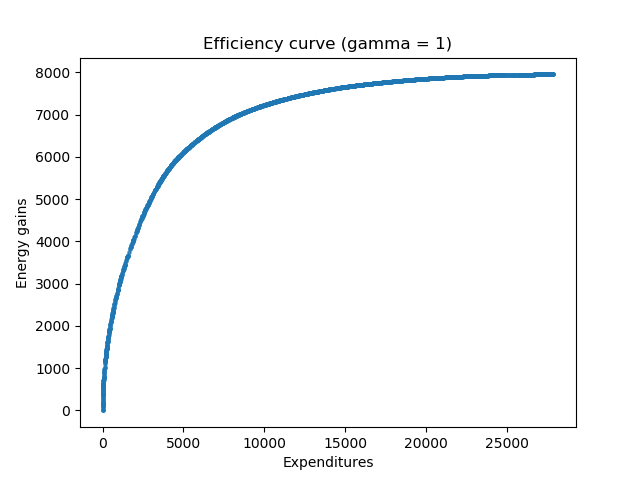
\includegraphics[scale=.7]{efficiency-curve.png}
\end{center}
\caption{Example of efficiency curve}
\label{fig:eff-curv}
\end{figure}

To draw an efficiency curve, we need to compute the expenditures $\delta(\mathbf{j}(t))$ at each state $\mathbf{j}(t)$:
\begin{equation}
	\delta(\mathbf{j}(t)) = \sum^{N}_{i=1} (V_0^i - V^i_{j(t)})
\end{equation}
and the energy gains $e(\mathbf{j}(t))$ at each iteration $t$:
\begin{equation}
	e(\mathbf{j}(t)) = \sum^{N}_{i=1} (e^i_0 - e^i_{j(t)}).
\end{equation}
We get as many pairs $(\delta, e)$ as there are iterations. Then, the efficiency curve can be drawn as a floor function.
\[ \text{[insert simple example of floor function]} \]

Consider the points $(\delta(\mathbf{j}(t-1)), e(\mathbf{j}(t-1)))$ and $(\delta(\mathbf{j}(t)), e(\mathbf{j}(t)))$.
The distance on the $x$-axis between those two points is $\delta(\mathbf{j}(t)) - \delta(\mathbf{j}(t-1))$, i.e. the incentive chosen at iteration $t$ by the algorithm.
The distance on the $y$-axis is $e(\mathbf{j}(t)) - e(\mathbf{j}(t-1))$, i.e. the energy gains induced by the jump at iteration $t$.
Therefore, the points on the graph are close to each other if the incentive and the energy gains of the jumps are small.

The slope of the line between the pair $(\delta(\mathbf{j}(t)), e(\mathbf{j}(t)))$ and the pair $(\delta(\mathbf{j}(s)), e(\mathbf{j}(s)))$ is equal to the efficiency of the jump from state $\mathbf{j}(t)$ to state $\mathbf{j}(s)$:
\begin{equation}
	\frac{e(\mathbf{j}(s)) - e(\mathbf{j}(t))}{\delta(\mathbf{j}(s)) - \delta(\mathbf{j}(t))} = \frac{e(\mathbf{j}(t) \rightarrow \mathbf{j}(s))}{\delta(\mathbf{j}(t) \rightarrow \mathbf{j}(s))} = \sigma(\mathbf{j}(t) \rightarrow \mathbf{j}(s)). 
\end{equation}

%increasing, concave


\section{Example}
\label{sec:Taxation}

The utility of alternative $j$ for individual $i$ after the taxation is
\[ \hat{V}^i_j = V^i_j - \tau(E^i_j - A). \]

Assume first that $\tau = 0.02$ and $A = 0$. The utilities before and after the taxation are reported in the tables 1 to 3.

\begin{table}[h]
	\centering
	\caption{Individual 1}
	\label{tab:label}
	\begin{tabular}{|c|c|c|c|c|}
		\hline
		Energy consumption ($E_j$) & Energy gains & Utility before & Tax & Utility after\\
		\hline
		500 & 0 & \textbf{10} & 10 & 0\\
		\hline
		400 & 100 & 9 & 8 & 1\\
		\hline
		290 & 210 & 8 & 5.8 & 2.2\\
		\hline
		205 & 295 & 7 & 4.1 & \textbf{2.9}\\
		\hline
		186 & 314 & 6 & 3.72 & 2.28\\
		\hline
		$\vdots$ & $\vdots$ & $\vdots$ & $\vdots$ & $\vdots$\\
		\hline
	\end{tabular}
\end{table}

\begin{table}[h]
	\centering
	\caption{Individual 2}
	\label{tab:label}
	\begin{tabular}{|c|c|c|c|c|}
		\hline
		Energy consumption ($E_j$) & Energy gains & Utility before & Tax & Utility after\\
		\hline
		500 & 0 & \textbf{10} & 10 & 0\\
		\hline
		410 & 90 & 9 & 8.2 & 0.8\\
		\hline
		390 & 110 & 8 & 7.8 & 0.2\\
		\hline
		265 & 235 & 7 & 5.3 & \textbf{1.7}\\
		\hline
		246 & 254 & 6 & 4.92 & 1.08\\
		\hline
		$\vdots$ & $\vdots$ & $\vdots$ & $\vdots$ & $\vdots$\\
		\hline
	\end{tabular}
\end{table}

\begin{table}[h]
	\centering
	\caption{Individual 3}
	\label{tab:label}
	\begin{tabular}{|c|c|c|c|c|}
		\hline
		Energy consumption ($E_j$) & Energy gains & Utility before & Tax & Utility after\\
		\hline
		500 & 0 & \textbf{10} & 10 & 0\\
		\hline
		430 & 70 & 9 & 8.6 & 0.4\\
		\hline
		365 & 135 & 8 & 7.3 & 0.7\\
		\hline
		300 & 200 & 7 & 6 & \textbf{1}\\
		\hline
		280 & 220 & 6 & 5.6 & 0.4\\
		\hline
		$\vdots$ & $\vdots$ & $\vdots$ & $\vdots$ & $\vdots$\\
		\hline
	\end{tabular}
\end{table}

With $\tau=0.02$ and $A=0$, everyone choose his fourth choice.

With a budget of $9$, the algorithm would give incentives such that all individuals are at their fourth choice. 
The efficiency of the last jump is 65 and the efficiency of the next jump is 19.
According to proposition \ref{propo2}, the MCP is equivalent to the algorithm in terms of allocation if $19 < 1/\tau \leq 65 ~\Leftrightarrow~ 0.015 \leq \tau < 0.053$.
With $\tau = 0.02$, this condition is met so the proposition is verified here.
\\

The income of the policy is $4.1 + 5.3 + 6 = 15.4$.

Total utility before the policy is $10 + 10 + 10 = 30$ and total utility after the policy is $2.9 + 1.7 + 1 = 5.6$.
To maintain utility constant before and after the policy, the government must give $30 - 5.6 = 24.4$ to the individuals.

Then, total cost of the policy is $24.4 - 15.4 = 9$.


\newpage

\end{document}
